%xelatex
\documentclass[11pt]{article}
\usepackage{amsfonts}
\usepackage{amsmath}
\usepackage{amssymb}
\usepackage[colorlinks]{hyperref}
\usepackage{bookmark}
\usepackage[dvipsnames]{xcolor}
\usepackage{soul}
\usepackage{fancybox}
\usepackage[most]{tcolorbox}
\usepackage{graphicx}
\usepackage{latexsym}
\usepackage{indentfirst}
\usepackage{listings}
\usepackage{multicol}
\usepackage{booktabs} % for tables
\setlength{\oddsidemargin}{.25in}
\setlength{\evensidemargin}{.25in}
\setlength{\textwidth}{6in}
\setlength{\topmargin}{-0.4in}
\setlength{\textheight}{8.5in}

\newtheorem{theorem}{Theorem}[section]
\newtheorem{fact}[theorem]{Fact}
\newtheorem{proposition}[theorem]{Proposition}
\newtheorem{lemma}[theorem]{Lemma}
\newtheorem{definition}[theorem]{Definition}
\newtheorem{corollary}[theorem]{Corollary}
\newtheorem{remark}[theorem]{Remark}
\newtheorem{claim}[theorem]{Claim}
\newtheorem{conjecture}[theorem]{Conjecture}
\newtheorem{assumption}[theorem]{Assumption}

\newcommand{\qed}{\hfill \ensuremath{\Box}}

\newenvironment{proof}{
\vspace*{-\parskip}\noindent\textit{Proof.}}{$\qed$

\medskip
}

\newcommand{\alg}[1]{\mathsf{#1}}
\newcommand{\Prover}{\alg{P}}
\newcommand{\Verifier}{\alg{V}}
\newcommand{\Simulator}{\alg{S}}
\newcommand{\PPT}{\alg{PPT}}
\newcommand{\isom}{\cong}
\newcommand{\from}{\stackrel{\scriptstyle R}{\leftarrow}}
\newcommand{\handout}[5]{
   \renewcommand{\thepage}{#1-\arabic{page}}
   \noindent
   \begin{center}
   \framebox{
      \vbox{
    \hbox to 5.78in { {\bf STAT 5310} \hfill #2 }
       \vspace{4mm}
       \hbox to 5.78in { {\Large \hfill #5  \hfill} }
       \vspace{2mm}
       \hbox to 5.78in { {\it #3 \hfill #4} }
      }
   }
   \end{center}
   \vspace*{4mm}
}

\newcommand{\ho}[5]{\handout{#1}{#2}{Instructor:
#3}{Scribe: #4}{Assignment #1: #5}}
\newcommand{\al}{\alpha}
\newcommand{\Z}{\mathbb Z}

\newcommand{\prob}[1]{
%\begin{center}
%	\noindent\doublebox{\parbox{.9\textwidth}{\large \bf #1}}
%\end{center}
\begin{tcolorbox}[colback=green!5!white,colframe=green!75!black]
#1
\end{tcolorbox}
}

\begin{document}

%\ho{3}{2024-04-02}{Jabed Tomal}{Hao Xu}{Assignment3}
Source code of this document:

\url{https://github.com/cld4h/DASC_6510_Assignment/tree/master/STAT_5310_AST3}

\section{Question 1}
\prob{
Let $x_1, x_2, \ldots, x_m$ is a random sample from a Poisson($\lambda$) distribution, where $\lambda \in \mathcal{R}$ is unknown. Determine/calculate/perform the:
\begin{multicols}{2}
\begin{enumerate}
\item Likelihood function, \item Log-likelihood function, \item Score equation, \item Fisher’s information, \item MLE, \item Second derivative test
\end{enumerate}
\end{multicols}
}

\begin{align*}
L(\lambda)
&= \prod_{i=1}^m P(X=x_i)\\
&= \prod_{i=1}^m \frac{e^{-\lambda}\lambda^{x_i}}{x_i!} \propto e^{-m\lambda} \lambda^{\sum_{i=1}^{m} x_i}\\
l(\lambda)
&= \sum_{i=1}^{m} \left( \ln\left( e^{-\lambda} \right) +\ln\left(  \lambda^{x_i} \right) - \ln\left( x_{i}! \right) \right) \\
&=  -m\lambda + \ln(\lambda)\sum_{i=1}^{m} x_{i} - \sum_{i=1}^{m}\ln\left( x_{i}! \right)\\
U(\lambda)=\frac{\partial l(\lambda)}{\partial \lambda}
&=-m+\frac{1}{\lambda}\sum_{i=1}^{m} x_{i}\\
I_n(\lambda) = \text{Var}_{\lambda}\{U(\lambda)\} 
&= -\text{E}_{\lambda}\{l''\left( \lambda \right) \} \\
&= -\text{E}_{\lambda}\{-\lambda^{-2}\sum_{i=1}^{m} x_{i}\}\\
&=\lambda^{-2} \text{E}_{\lambda}\left( \sum_{i=1}^{m} x_i \right) =\lambda^{-2}\cdot m \lambda\\
&= \frac{m}{\lambda}\\
\hat{\lambda}_\text{MLE} &= \frac{\sum_{i=1}^{m} x_{i}}{m}\\
\end{align*}

\[
\forall \lambda \in \mathcal{R}\backslash\{0\}, x_{i} \in N,  l''(\lambda)= -\lambda^{2}\sum_{i=1}^{m} x_{i} < 0
\] 

\section{Question 2}
\prob{
If $x_1,x_2,\ldots,x_{n}$ is a random sample from an $N(\mu_0, \sigma^{2})$ distribution, where $\sigma^{2}>0$ is unknown and $\mu_0$ is known, then determine the MLE of $\sigma^2$.
}

\begin{align*}
L\left( \sigma^2|x_{i}, \mu_0 \right) &= \prod_{i=1}^{n}\frac{1}{\sigma\sqrt{2\pi}}\exp{\{-\frac{\left( x_i-\mu_0 \right)^{2}}{2\sigma^2} \}}\\
				      &= (2\pi\sigma^2)^{-\frac{n}{2}}\exp{\{-\sum_{i=1}^{n}\frac{\left( x_i-\mu_0 \right)^{2}}{2\sigma^2} \}}\\
l\left( \sigma^2|x_{i}, \mu_0 \right) &= \sum_{i=1}^{n} \left(  -\frac{1}{2}\ln(2\pi\sigma^2 )-\frac{\left( x_i-\mu_0 \right)^{2}}{2\sigma^2} \right) \\
U\left( \sigma^2 \right)  = \frac{\partial l(\sigma^2,x_{i},\mu_0)}{\partial \sigma^2}
&=-\frac{n}{2\sigma^2}+\frac{1}{2(\sigma^2)^2}\sum_{i=1}^{n}(x_i-\mu_0)^2\\
\text{Solve }\frac{\partial l(\sigma^2,x_{i},\mu_0)}{\partial \sigma^2} &= 0 \text{ for $\sigma^2$}\\
\frac{n}{2\sigma^2}&=\frac{1}{2(\sigma^2)^2}\sum_{i=1}^{n}(x_i-\mu_0)^2\\
{n}{\sigma^2}&=\sum_{i=1}^{n}(x_i-\mu_0)^2\\
\therefore\hat{\sigma}_{\text{MLE}}^2&=\frac{1}{n}\sum_{i=1}^{n}(x_i-\mu_0)^2\\
\end{align*}

The second derivative of likelihood function is
\begin{align*}
\frac{\partial^2 l(\sigma^2,x_{i},\mu_0)}{\partial^2 (\sigma^2)}
&=\frac{n}{2(\sigma^2)^2}-\frac{2}{2(\sigma^2)^3}\sum_{i=1}^{n}(x_i-\mu_0)^2\\
&=\frac{1}{(\sigma^2)^3}(\frac{n\sigma^2}{2}-\sum_{i=1}^{n}(x_i-\mu_0)^2)\\
\end{align*}

when $\frac{n\sigma^2}{2}-\sum_{i=1}^{n}(x_i-\mu_0)^2 < 0 \Leftrightarrow \sigma^2<\frac{2\sum_{i=1}^{n}(x_i-\mu_0)^2}{n}$, the likelihood function gets local maximum value at $\hat{\sigma}^2=\frac{1}{n}\sum_{i=1}^{n}(x_i-\mu_0)^2$, when $\sigma^2>\frac{2\sum_{i=1}^{n}(x_i-\mu_0)^2}{n}$, even though the $U(\sigma^2)$ is increasing, it is always a negative value ( we have only 1 solution for the equation $U(\sigma^2) = 0$, so the likelihood function is monotonically decreasing when $\sigma^2 > \frac{1}{n}\sum_{i=1}^{n} \left( x_i-\mu_0 \right) ^2$, so the local maximum value is the global maximum value.

\section{Question 3}

\prob{Suppose that in a population of students in a course with a large enrollment, the mark, out of 100, on a final exam is approximately distributed $N (\mu, \sigma^2 = 9)$. The instructor places the prior $\mu \sim N(\mu_0=65,\tau_0^2=1)$ on the unknown parameter. A sample of 10 marks is obtained as given below.

\begin{center}
\begin{tabular}{cccccccccc}
\hline
46 & 68 & 34 & 86 & 75 & 56 & 77 & 73 & 53 & 64\\
\hline
\end{tabular}
\end{center}

(a) Determine the posterior mode and a 0.95-credible interval for $\mu$. What does this interval tell you about the accuracy of the estimate?

(b) Use the 0.95-credible interval for $\mu$ to test the hypothesis $H_0: \mu = 65$
}

Claim: The posterior distribution of $\{\mu|y_1,\ldots,y_n,\sigma^2\}$ follows a Normal distribution.

Proof:

The sampling distribution of $\{y_1,\ldots,y_n | \mu, \sigma^2\}$ is: 

\begin{align*}
p(y_1,\ldots,y_n|\mu,\sigma^2) 
&= \prod_{i=1}^{n} \frac{1}{\sqrt{2\pi\sigma^2} }\exp\left( -\frac{(y_i-\mu)^2}{2\sigma^2}  \right)   \\
&=(2\pi\sigma^2)^{-\frac{n}{2}}\exp\left( -\frac{1}{2\sigma^2}\sum_{i=1}^{n} \left(y_i-\mu \right) ^2 \right) 
.\end{align*}

The prior distribution of $\{\mu|\sigma^2,\mu_0,\tau_0^2\}$ is:

\begin{align*}
p(\mu|\sigma^2,\mu_0,\tau_0^2)
&=\frac{1}{\sqrt{2\pi\sigma^2}} \exp\left( -\frac{\left( \mu-\mu_0 \right)^2 }{2\tau_0^2} \right)
.\end{align*}

The posterior distribution of $\{\mu|y_1,\ldots,y_n,\sigma^2,\mu_0,\tau_0^2\}$ is:

\begin{align*}
p(\mu|y_1,\ldots,y_n, \sigma^2, \mu_0, \tau_0^2) 
&= p(\mu|\sigma^2)\cdot p(y_1,\ldots,y_n|\mu,\sigma^2)\\
&\propto \exp\left( -\frac{\left( \mu-\mu_0 \right)^2 }{2\tau_0^2} \right)\cdot \exp\left( -\frac{\sum_{i=1}^{n} \left(y_i-\mu \right) ^2}{2\sigma^2} \right) \\
&= \exp\left[ -\frac{1}{2}\left( \frac{\left( \mu-\mu_0 \right)^2 }{\tau_0^2} + \frac{\sum_{i=1}^{n} \left(y_i^2-2y_i\mu+\mu^2 \right) }{\sigma^2} \right)\right] \\
&= \exp\left[ -\frac{1}{2}\left( \frac{\left( \mu^2-2\mu\mu_0+\mu_0^2 \right) }{\tau_0^2} + \frac{\left(\sum_{i=1}^{n} y_i^2-2\mu\sum_{i=1}^{n} y_i+n\mu^2 \right) }{\sigma^2} \right)\right] \\
&= \exp\left[ -\frac{1}{2}\left( \frac{\tau_0^2 \left(\sum_{i=1}^{n} y_i^2-2\mu\sum_{i=1}^{n} y_i+n\mu^2 \right)+ \sigma^2 \left( \mu^2-2\mu\mu_0+\mu_0^2 \right)}{\sigma^2\tau_0^2} \right)\right] \\
&\propto \exp\left[ -\frac{1}{2}\left( \frac{(n\tau_0^2+\sigma^2)\mu^2 - 2\mu\left( \tau_0^2 \sum_{i=1}^{n} y_i + \sigma^2\mu_0 \right) }{\sigma^2\tau_0^2} \right)\right] \\
&\propto \exp\left[ -\frac{1}{2}\left( \frac{(n\tau_0^2+\sigma^2)(\mu-\frac{ \tau_0^2 \sum_{i=1}^{n} y_i + \sigma^2\mu_0 }{n\tau_0^2+\sigma^2})^2 }{\sigma^2\tau_0^2} \right)\right] \\
\end{align*}

Get the normalizing coefficient $C$ for this normal distribution:

\begin{align*}
\because \int_{-\infty}^{\infty}p(\mu|y_1,\ldots,y_n, \sigma^2, \mu_0, \tau_0^2) d \mu &= \int_{-\infty}^{\infty}C\cdot \exp\left[ -\frac{1}{2}\left( \frac{(n\tau_0^2+\sigma^2)(\mu-\frac{ \tau_0^2 \sum_{i=1}^{n} y_i + \sigma^2\mu_0 }{n\tau_0^2+\sigma^2})^2 }{\sigma^2\tau_0^2} \right)\right] d \mu = 1 \\
\therefore C \sqrt{2\pi \frac{\sigma^2\tau_0^2}{n\tau_0^2+\sigma^2}}\cdot &\int_{-\infty}^{\infty} \frac{1}{\sqrt{2\pi \frac{\sigma^2\tau_0^2}{n\tau_0^2+\sigma^2}} }\exp\left[ -\frac{1}{2}\left( \frac{(n\tau_0^2+\sigma^2)(\mu-\frac{ \tau_0^2 \sum_{i=1}^{n} y_i + \sigma^2\mu_0 }{n\tau_0^2+\sigma^2})^2 }{\sigma^2\tau_0^2} \right)\right] d \mu = 1\\
									      C&=\frac{1}{\sqrt{2\pi \frac{\sigma^2\tau_0^2}{n\tau_0^2+\sigma^2}} }
\end{align*}

$\therefore \{\mu|y_1,\ldots,y_n, \sigma^2, \mu_0, \tau_0^2\} \sim N(\frac{ \tau_0^2 \sum_{i=1}^{n} y_i + \sigma^2\mu_0 }{n\tau_0^2+\sigma^2}, \frac{\sigma^2\tau_0^2}{n\tau_0^2+\sigma^2})$

The posterior mode of $\{\mu|y_1,\ldots,y_n, \sigma^2, \mu_0, \tau_0^2\}$ is $\frac{ \tau_0^2 \sum_{i=1}^{n} y_i + \sigma^2\mu_0 }{n\tau_0^2+\sigma^2} = \frac{1\times632+9\times 65}{10\times 1+9} = \frac{1217}{19} = 64.05263$

The posterior variance of $\{\mu|y_1,\ldots,y_n, \sigma^2, \mu_0, \tau_0^2\}$ is $\frac{\sigma^2\tau_0^2}{n\tau_0^2+\sigma^2} = \frac{9}{19} = 0.4736842$ 

The 0.95-credible interval for $\{\mu|y_1,\ldots,y_n, \sigma^2, \mu_0, \tau_0^2\}$ is:
\begin{align*}
&[64.05263+\text{qnorm(0.025)}\sqrt{0.4736842}, \quad 64.05263+\text{qnorm(0.975)}\sqrt{0.4736842} ] \\
=& [62.70369, 65.40157]
.\end{align*}

\begin{figure}[htpb]
	\centering
	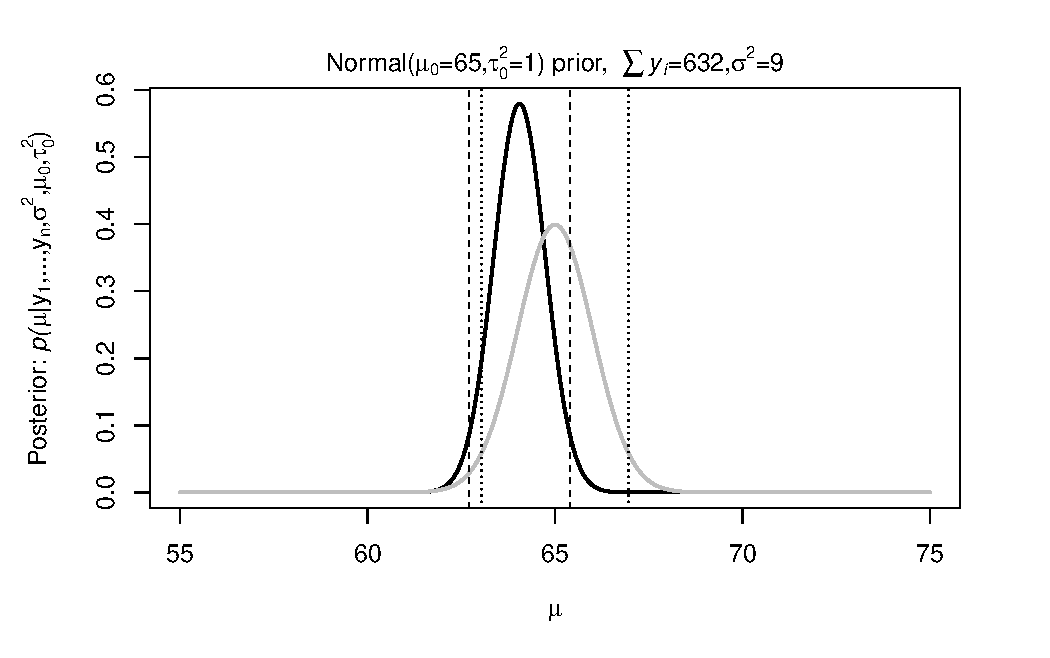
\includegraphics[width=\textwidth]{Ast3-Q3.pdf}
	\caption{Prior (in gray) and Posterior (in black) distribution of $\mu$.}
	\label{fig:Ast3-Q3-pdf}
\end{figure}

As shown in Figure~\ref{fig:Ast3-Q3-pdf}, the posterior distribution of $\mu$ is plotted in Black, and the 95\% credible interval is ploted in dashed lines. The prior distribution of $\mu$ is plotted in gray, and the 95\% credible interval of prior $\mu$ is plotted in dotted lines. We can see that the credible intervals is narrower for the posterior distribution compared to prior. Thus, we can say that the accuracy is improved.

Also if we use classical frequentist method, the confidence interval we get is:

\begin{align*}
& \left[\overline{y}-\frac{\sigma}{\sqrt{n_y}}, \overline{y}+\frac{\sigma}{\sqrt{n_y}} \right]\\
=& \left[63.2-\frac{3}{\sqrt{10}}, 63.2+\frac{3}{\sqrt{10}}\right]\\
=& \left[62.25132, 64.14868\right]
\end{align*}

Therefore, we have a very good example of bayesian method NOT rejecting $H_0: \mu = 65$ (because $65 \in [62.70369, 65.40157]$) but classical frequentist method will reject the $H_0: \mu = 65$ ($65 \notin \left[62.25132, 64.14868\right]$).

\section{Question 4}

\prob{
Tumor counts: A cancer laboratory is estimating the rate of tumorigenesis in two strains of mice, $A$ and $B$. They have tumor count data for 10 mice in strain $A$ and 13 mice in strain $B$. Type $A$ mice have been well studied, and information from other laboratories suggests that type $A$ mice have tumor counts that are approximately Poisson-distributed with a mean of 12. Tumor count rates for type $B$ mice are unknown, but type $B$ mice are related to type $A$ mice. The observed tumor counts for the two populations are
\begin{align*}
	\mathbf{y}_A &= (12, 9, 12, 14, 13, 13, 15, 8, 15, 6);\\
	\mathbf{y}_B &= (11, 11, 10, 9, 9, 8, 7, 10, 6, 8, 8, 9, 7)
\end{align*}


(a) Find the posterior distributions, means, variances and 95\% quantile based confidence intervals for $\theta_A$ and $\theta_B$ , assuming a Poisson sampling distribution for each group and the following prior distribution:
$\theta_A \sim Gamma(\alpha_A = 120, \beta_A=10), \theta_B \sim Gamma(\alpha_B = 12, \beta_B = 1), \pi(\theta_A, \theta_B ) = \pi(\theta_A)\times \pi(\theta_B).$

(b) Compute and plot the posterior expectation of $\theta_B$ under the prior distribution $\theta_B \sim \text{Gamma}(12\times n_0,n_0)$ for each value of $n_0 \in \{1,2,\ldots,50\}$. Describe what sort of prior beliefs about $\theta_B$ would be necessary in order for the posterior expectation of $\theta_B$ to be close to that of $\theta_A$. 

(c)Should knowledge about population $A$ tell us anything about population $B$? Discuss whether or not it makes sense to have $\pi(\theta_A, \theta_B) = \pi(\theta_A)\times \pi(\theta_A)$.
}

Claim: The posterior distribution of $\{\theta|y_1,\ldots,y_n,\alpha, \beta\} \sim \text{Gamma}\left( \alpha, \beta \right) $ 

Proof:

Prior distribution of $\{\theta|\alpha, \beta\}$ is: 

\begin{align*}
p(\theta|\alpha, \beta)
&= \frac{\beta^\alpha}{\Gamma(\alpha)}\cdot \theta^{\alpha-1}e^{-\beta\theta}
\end{align*}

The sampling distribution of $\{y_1,\ldots,y_n|\theta\}$ is:

\begin{align*}
p(y_1,\ldots,y_n|\theta)
&=\prod_{i=1}^{n} \frac{1}{y_i!}\theta^{y_i}e^{-\theta}\\
&=c(y_1,\ldots,y_n)\cdot \theta^{\sum_{i=1}^{n} y_i}e^{-n\theta}\\
\end{align*}

The posterior distribution of $\{\theta|y_1,\ldots,y_n, \alpha, \beta\}$ is:

\begin{align*}
p(\theta|y_1,\ldots,y_n, \alpha, \beta)
&=p(\theta|\alpha, \beta)\cdot p(y_1,\ldots,y_n|\theta)\\
&=\frac{\beta^\alpha}{\Gamma(\alpha)}\cdot \theta^{\alpha-1}e^{-\beta\theta}\cdot c(y_1,\ldots,y_n)\cdot \theta^{\sum_{i=1}^{n} y_i}e^{-n\theta}\\
&\propto \theta^{\alpha+\sum_{i=1}^{n} y_i -1}e^{-(\beta+n)\theta}
\end{align*}

$\therefore \{\theta|y_1,\ldots,y_n, \alpha, \beta\} \sim \text{Gamma}(\alpha+\sum_{i=1}^{n} y_i, \beta+n)$

\begin{itemize}
\item The mean of a Gamma distribution $f(\theta) = \frac{\beta^{\alpha}}{\Gamma(\alpha)}\theta^{\alpha-1}e^{-\beta \theta}$ is $\frac{\alpha}{\beta}$
\item The variance of a Gamma distribution $f(\theta) = \frac{\beta^{\alpha}}{\Gamma(\alpha)}\theta^{\alpha-1}e^{-\beta \theta}$ is $\frac{\alpha}{\beta^2}$
\end{itemize}

\begin{table}[htpb]
	\centering
	\caption{part (a) answer}
	\label{tab:label}
	\begin{tabular}{lll}
	\toprule
	Mean: $\frac{\alpha+\sum_{i=1}^{n} y_i}{\beta+n}$  & Variance: $\frac{\alpha+\sum_{i=1}^{n} y_i}{(\beta+n)^2}$ & 95\% quantile based credible interval\\
	\midrule
	11.85& 0.5925& [10.38924, 13.40545]\\
	8.928571&0.6377551&[7.4320, 10.560308]\\
	\bottomrule
	\end{tabular}
\end{table}

\begin{figure}[htpb]
	\centering
	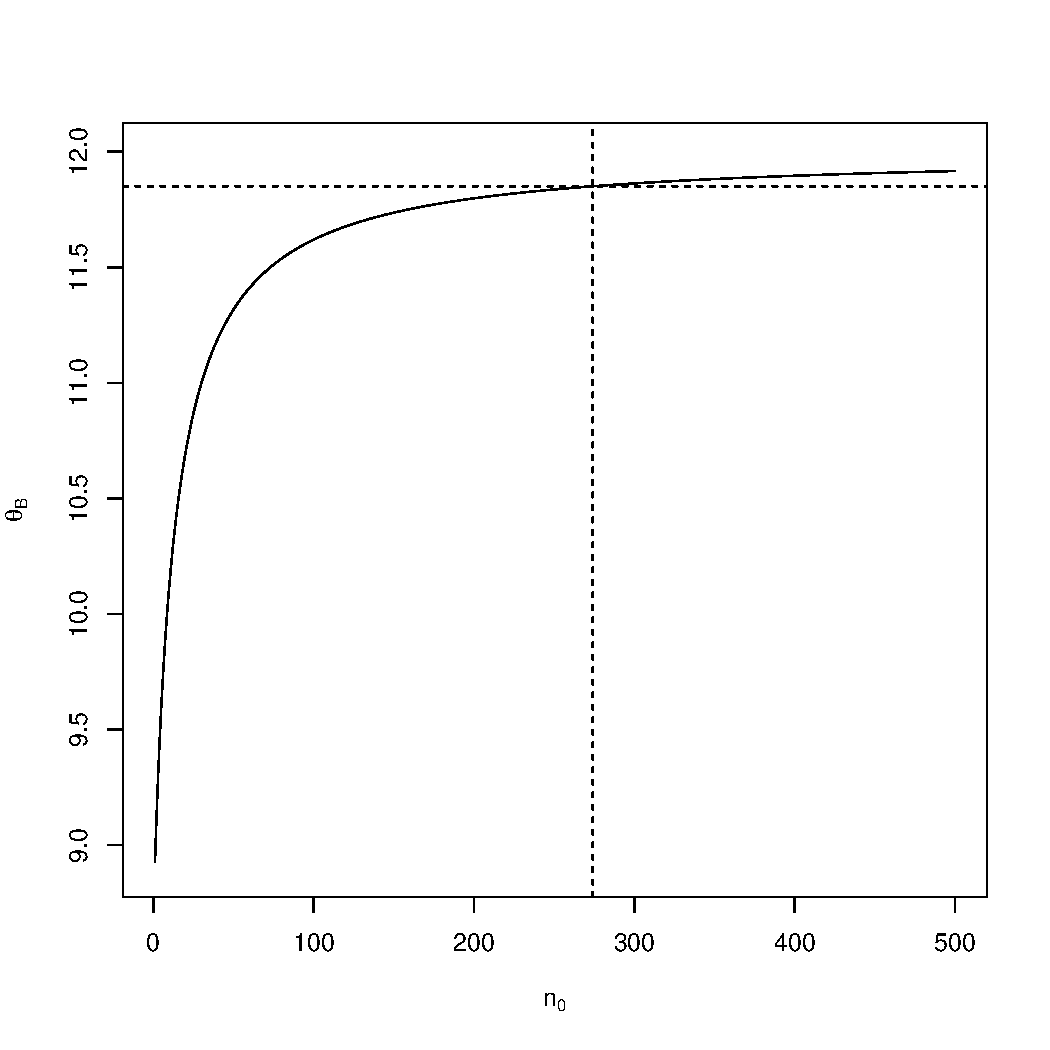
\includegraphics[width=0.8\textwidth]{Ast3-Q4-partb.pdf}
	\caption{Mean of $\theta_B$ with respect to different $n_0$}
	\label{fig:Ast3-Q4-partb-pdf}
\end{figure}

Figure~\ref{fig:Ast3-Q4-partb-pdf} plots the relationship between $\theta_B$ and $n_0$. The larger the $n_0$, the stronger the belief, the more closer the posterior expectation of $\theta_B$ is to that of $\theta_A$. When $n_0 = 274$, the two values are the same (the cross point of the two dashed line in Figure~\ref{fig:Ast3-Q4-partb-pdf}).

Because type B mice are related to type A mice, so knowledge about ppopulation A should tell us something about population B. Having $\pi(\theta_A,\theta_B) = \pi(\theta_A) \times \pi(\theta_B)$ is assuming the prior distribution of $\theta_A$ annd $\theta_B$ to be independent, which prevent us from borrowing information from population A to population B. So it doesn't make sence.

\newpage
\section{Question 5}
\prob{
Let $f(x) = \text{exp}(-x^{4}-x^{6}-x^{8})$ for $x \in \mathcal{R}^1$ and let $K = \frac{1}{\int_{-\infty}^{\infty} f(x) dx}$. Describe in detail a Metrpolis-Hastings algorithm for the distribution having density $Kf(x)$, which uses proposal distributions (a)$N (\mu = x, \sigma^2 = 1)$ and (b)N $(\mu = x, \sigma^2 = 10)$.

(a) By producing traceplots, compare and contrast your experience in (a) and (b).

(b) Calculate $E(X)$ and $\text{Var}(X)$ for the distribution of $X \sim Kf(x)$
}

\begin{tcolorbox}[colback=blue!5!white,colframe=blue!75!black,title=Metropolis-Hastings Algorithm]
The Metropolis-Hastings algorithm is a Markov chain Monte Carlo (MCMC) method used for sampling from a probability distribution that is difficult to sample directly. It is particularly useful for sampling from high-dimensional distributions, such as posterior distributions in Bayesian inference.

Let \( \pi(x) \) be the target distribution from which we want to sample, and let \( q(x' \, | \, x) \) be a proposal distribution that generates a candidate sample \( x' \) given the current sample \( x \). The algorithm proceeds as follows:

\begin{enumerate}
    \item Initialize the Markov chain at some initial state \( x_0 \).
    \item For each iteration \( t \):
    \begin{enumerate}
        \item Generate a candidate sample \( x' \) from the proposal distribution \( q(x' \, | \, x_t) \).
        \item Calculate the acceptance probability:
        \[
        \alpha(x_t, x') = \min\left\{1, \frac{\pi(x') \, q(x_t \, | \, x')}{\pi(x_t) \, q(x' \, | \, x_t)}\right\}
        \]
        \item Generate a uniform random number \( u \) from the interval [0, 1].
        \item If \( u \leq \alpha(x_t, x') \), accept the candidate sample \( x' \) by setting \( x_{t+1} = x' \); otherwise, set \( x_{t+1} = x_t \).
    \end{enumerate}
\end{enumerate}


The resulting sequence of samples \( x_0, x_1, x_2, \ldots \) (often correlated) forms a Markov chain whose stationary distribution is \( \pi(x) \). By discarding an appropriate "burn-in" period and thinning the samples, one can obtain samples approximately drawn from the target distribution.

\end{tcolorbox}

\begin{tcolorbox}[colback=blue!5!white,colframe=blue!75!black,title=Metropolis Algorithm]
When $q$ is symmetric proposal distribution, $q\left( x|y \right) =q\left( y|x \right) $,  the expression for the acceptance ratio $\alpha\left( x_t, x' \right) $ simplifies to: 
\[
\alpha\left( x_t, x' \right) = \text{min}\left\{1, \frac{\pi(x')}{\pi(x_t)}\right\}
.\] 

Then Metropolis-Hastings algorithm simplifies to Metropolis algorithm. A common choice for $q(y|x)$ is $N(x, \tau^2)$ for some $\tau>0$. This means that the proposal is drawn from a Normal distribution centered at the current value.
\end{tcolorbox}

The histograms of the M-H sampled data are shown in Figure~\ref{fig:Ast3-Q5-hist-pdf};
The traceplots are shown in Figure~\ref{fig:Ast3-Q5-traceplots-pdf};
I also plotted the Stationarity boxplots and Autocorrelation functions values in Figure~\ref{fig:Ast3-Q5-stationarity-plot-pdf} and Figure~\ref{fig:Ast3-Q5-acf-plot-pdf}

From the program output, we know that the accept rate for proposal a is 0.517, and for proposal b it is 0.1897. We say that the accept rate for proposal a is nice because it's neither too high (which would result in slow mixing speed) or too low (wich might result in inefficient exploration). However, for proposal b, we can see from the traceplot it's more sparsely distributed compared to proposal a. This indicate that the exploration of probability space is inefficient.

We can also see from the stationarity plot (Figure~\ref{fig:Ast3-Q5-stationarity-plot-pdf} that chain a is more stable than chain b. And from the autocorrelation function plot (Figure~\ref{fig:Ast3-Q5-acf-plot-pdf} we can see that proposal b has a stronger autocorrelation between successive samples.

For part (b), we use the sampled data from proposal a to calculate $E(X)$ and $\text{Var}(X)$:

$E(X): -0.002967374$

$\text{Var}(X): 0.2187539 $

\begin{figure}[htpb]
	\centering
	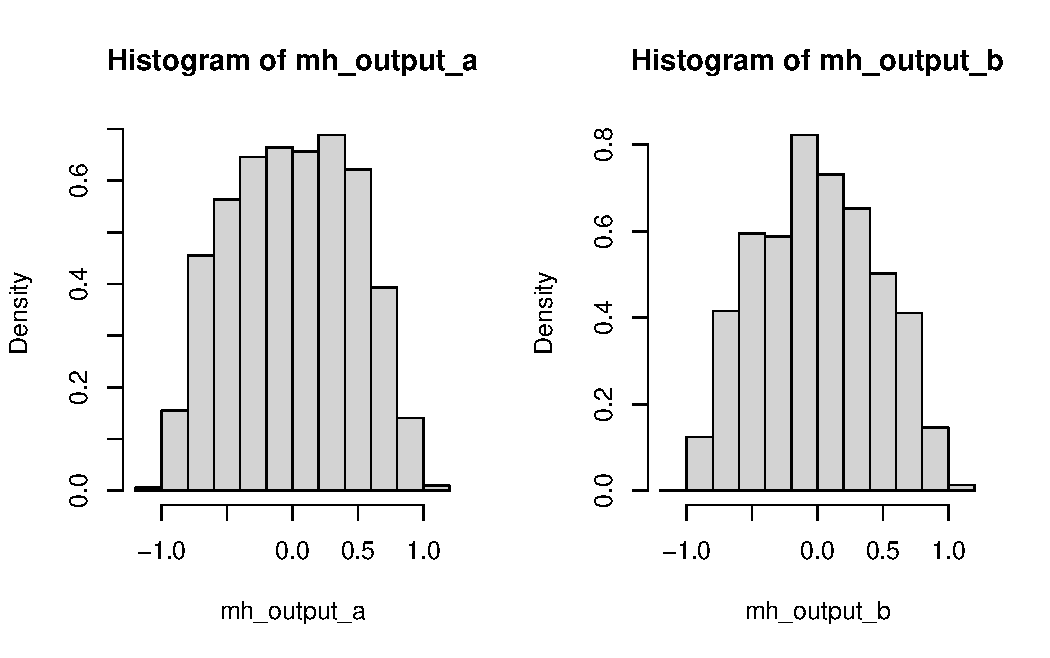
\includegraphics[width=0.8\textwidth]{Ast3-Q5-hist.pdf}
	\caption{Histogram of the M-H sampled data}
	\label{fig:Ast3-Q5-hist-pdf}
\end{figure}

\begin{figure}[htpb]
	\centering
	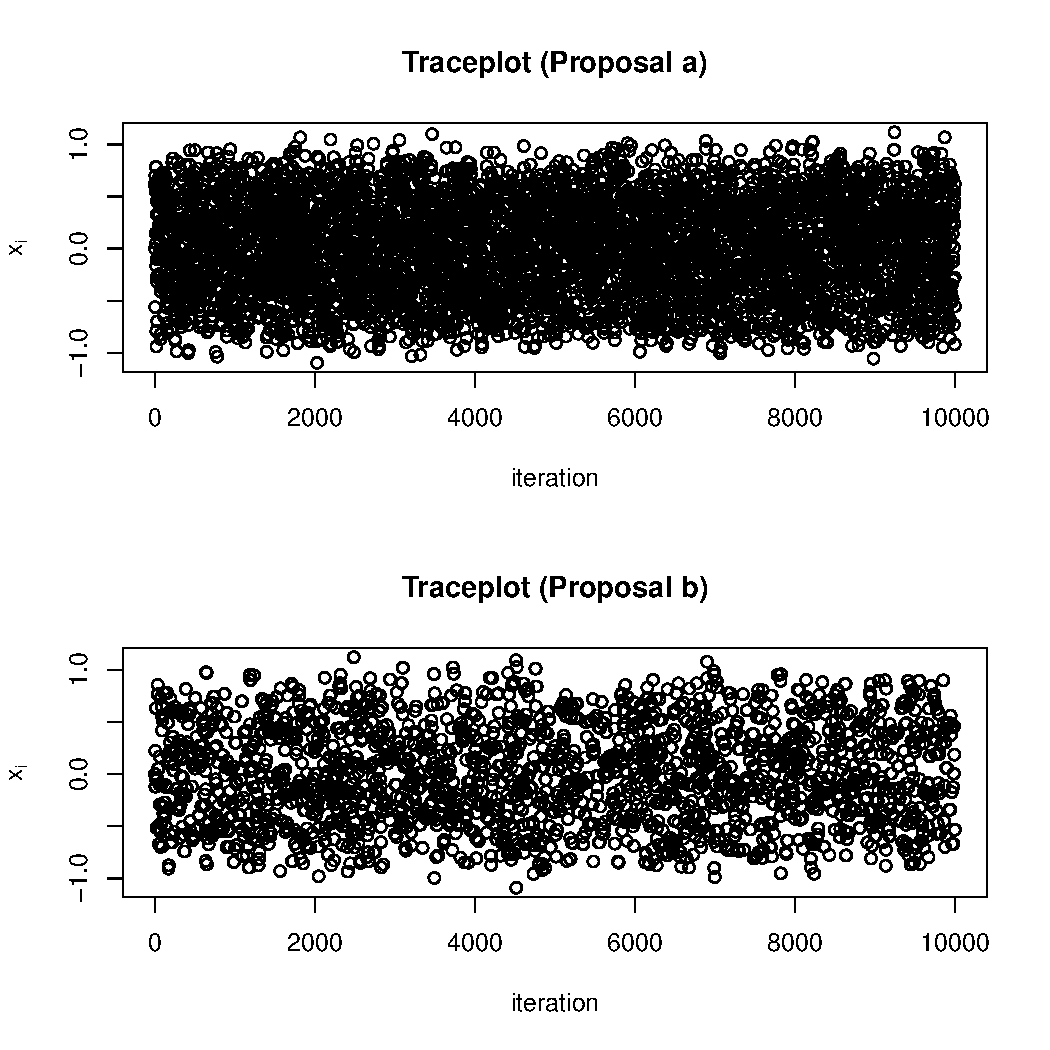
\includegraphics[width=0.8\textwidth]{Ast3-Q5-traceplots.pdf}
	\caption{Traceplot of the M-H sampled data}
	\label{fig:Ast3-Q5-traceplots-pdf}
\end{figure}

\begin{figure}[htpb]
	\centering
	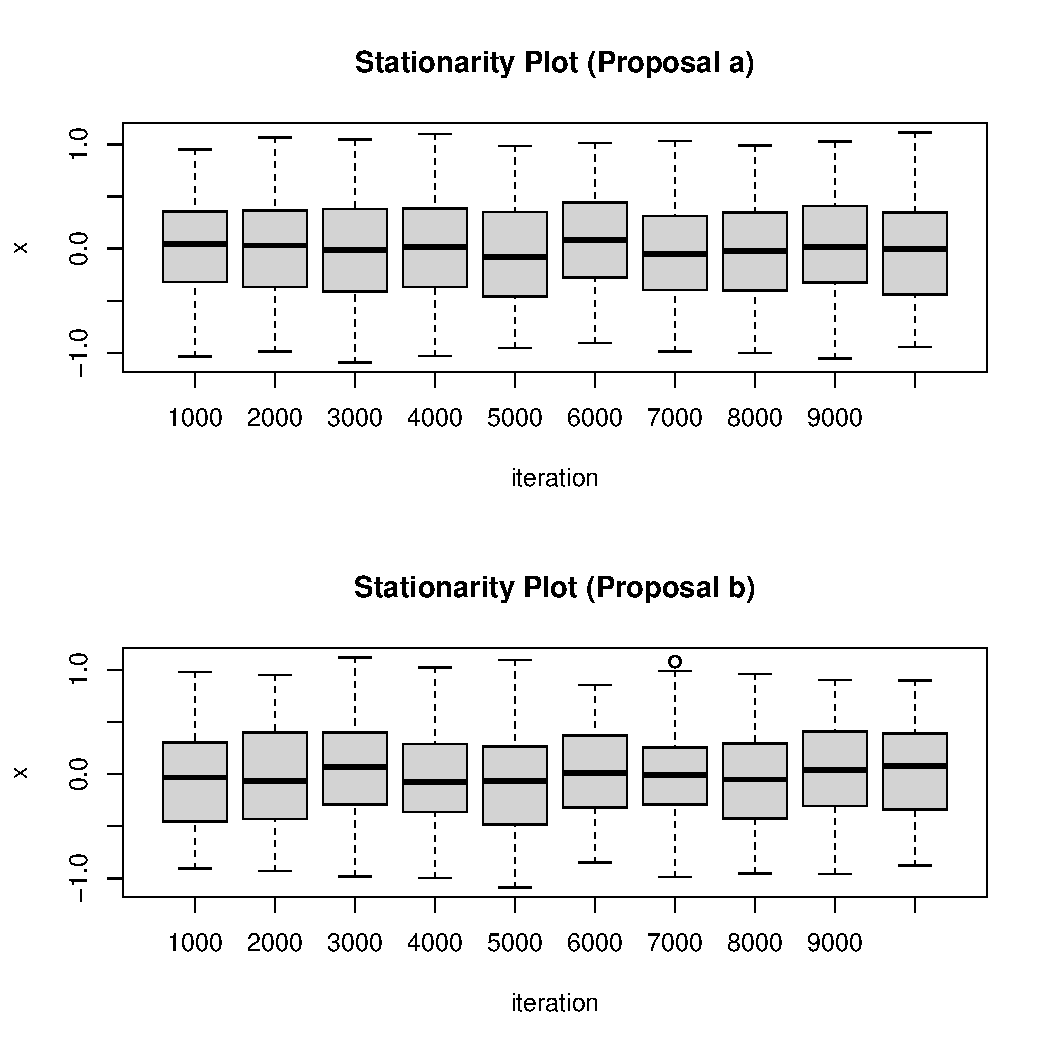
\includegraphics[width=0.8\textwidth]{Ast3-Q5-stationarity-plot.pdf}
	\caption{Stationarity plots of the M-H sampled data}
	\label{fig:Ast3-Q5-stationarity-plot-pdf}
\end{figure}

\begin{figure}[htpb]
	\centering
	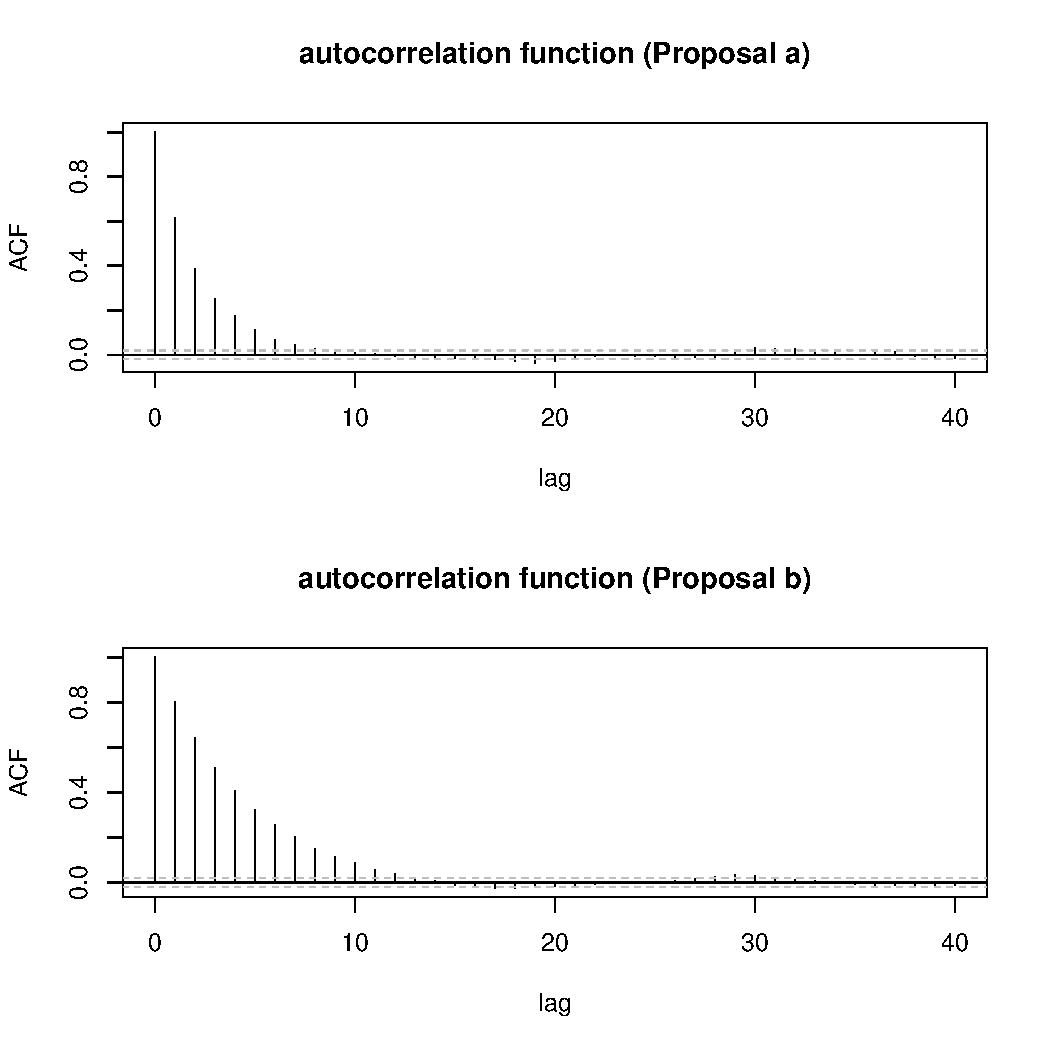
\includegraphics[width=0.8\textwidth]{Ast3-Q5-acf-plot.pdf}
	\caption{Autocorrelation plots of the M-H sampled data}
	\label{fig:Ast3-Q5-acf-plot-pdf}
\end{figure}

\end{document}
